\[
\pi(x) = \lfloor x \rfloor - \sum_{i=1}^a\left\lfloor\frac{x}{p_i}\right\rfloor + \sum_{1\leq i\leq j\leq a}\left\lfloor\frac{x}{p_ip_j}\right\rfloor-\ldots+\frac{1}{2}(b+a-2)(b-a+1)-\sum_{a<i\leq b}\pi\left(\frac{x}{p_i}\right) - \sum_{i=a+1}^c \sum_{j=i}^{b_i}\left[\pi\left(\frac{x}{p_ip_j}\right)-(j-1)\right],
a=\pi\left(x^{1/4}\right), b=\pi\left(x^{1/2}\right), 
b_i=\pi\left(\sqrt{x/p_i}\right), 
c=\pi\left(x^{1/3}\right)
\]

\begin{minipage}[t]{.47\textwidth}
$\displaystyle C_n=\binom{2n}{n}-\binom{2n}{n+1}=\frac{1}{n+1}\binom{2n}{n};
C_{n+1}=\sum_{i=0}^n C_iC_{n-i}=\frac{2(2n+1)}{n+2}C_n$

$\displaystyle C=1, 1, 2, 5, 14, 42, 132, 429, 1430, 4862, 16796, 58786, 208012, 742900, 2674440$

Number of permutations of length $n$ with $k$ cycles: \[s(n+1,k)=ns(n,k)+s(n,k-1)\]

Number of ways to partition a set of $n$ labelled objects into $k$ nonempty subsets: \[S(n,k)=\frac{1}{k!}\sum_{j=0}^k(-1)^{k-j}\binom{k}{j}j^n=kS(n-1,k)+S(n,k-1)\]

\[H_n=\sum_{k=1}^n\frac{1}{k}\approx\ln n+\gamma+\frac{1}{2n}-\frac{1}{12n^2}+\frac{1}{120n^4}-\frac{1}{252n^6}+\ldots\]
\[\frac{1}{2(n+1)}<H_n-\ln n-\gamma<\frac{1}{2n};
\frac{1}{24(n+1)^2}<H_n-\ln\left(n+\frac{1}{2}\right)-\gamma<\frac{1}{24n^2}\]
\[\gamma=0.57721566490153286060651209008240243104215933593992\]

Sphere: $\displaystyle V=\frac{4}{3}\pi r^3; A=4\pi r^2$

$\displaystyle V=\frac{\pi h}{6}\left(3a^2+h^2\right); A=2\pi rh=2\pi r^2\left(1-\cos\theta\right)=\pi\left(a^2+h^2\right);r=\frac{a^2+h^2}{2h}$

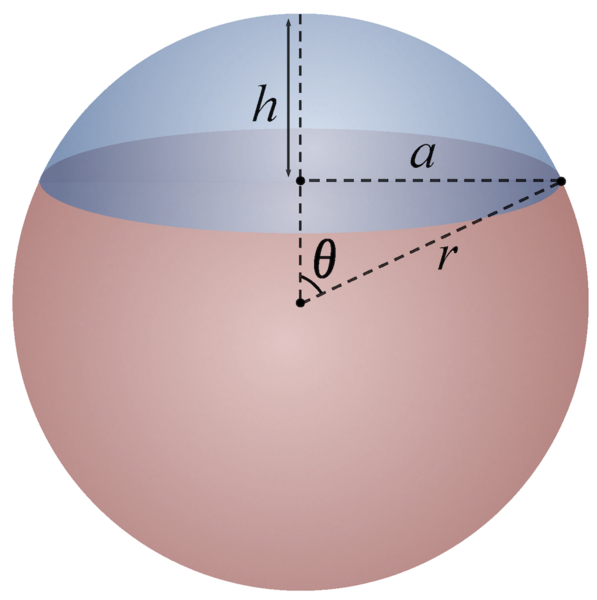
\includegraphics{SphericalCap.png}
\end{minipage}%
\begin{minipage}[t]{.47\textwidth}
Maximum Flows with Edge Demands: $\displaystyle c'(s'\rightarrow v)=\sum_{u\in V}d(u\rightarrow v)$, $\displaystyle c'(v\rightarrow t')=\sum_{w\in V}d(v\rightarrow w)$, $\displaystyle c'(u\rightarrow v)=c(u\rightarrow v)-d(u\rightarrow v)$, $\displaystyle c'(t\rightarrow s)=\infty$.
If feasible: $c_f(u\rightarrow v)=c(u\rightarrow v)-f(u\rightarrow v)$ if $u\rightarrow v\in E$; $f(v\rightarrow u)-d(v\rightarrow u)$ if $v\rightarrow u\in E$, $0$ otherwise.
\end{minipage}